\documentclass{article}
\usepackage[portuges]{babel}
\usepackage{epsfig,subfigure,cite,graphicx}
\usepackage{indentfirst}
\setlength{\parindent}{20pt}
\usepackage[cmex10]{amsmath}
\usepackage[left=2.5cm,top=2.5cm,right=2.5cm,bottom=2.5cm]{geometry}
\usepackage{enumitem}
% load package with ``framed'' and ``numbered'' option.
\usepackage[framed,numbered,autolinebreaks,useliterate]{mcode}
\renewcommand{\lstlistingname}{Código}
% something NOT relevant to the usage of the package.
\usepackage{url}
\setlength{\parindent}{0pt}
\setlength{\parskip}{18pt}
\title{CONTROLE 1}

% //////////////////////////////////////////////////


\begin{document}


\section*{AVALIAÇÃO 2 - CONTROLE 1}

\indent Aluno: Vitor de Sousa França\\
\indent Matrícula: 20180041455\\
\indent 27 de Outubro de 2021\\

\section*{Problemas PID: }
    Considerando-se o sistema:  
    \begin{equation*}
        G = \frac{0.25(K_d s^2 + K_p s +K_i)}{s(s+1)(s+5)}
    \end{equation*}
    
    Em que $K_d = 150.88$, $K_p = 1373.92$ e $K_i = 5000$
    
    \subsection*{a) Utilize o MATLAB e realize as simulações do sistema em malha 
    fechada no domínio do tempo contínuo.}

        Primeiro, foram definidas as funções de transferência (FT) da planta, do controlador e então obteve-se 
        o ganho em malha aberta (MA) e em malha fechada (MF), posto que esse conjunto de FT serão utilizados por várias
        questões. O bloco de código \ref{DefFT} apresenta

        \begin{lstlisting}[language=Matlab,label=DefFT,caption=Definindo FTs]
%Planta
Nump = 0.25;
Denp = conv([1 1], [1 5]);
H = tf(Nump, Denp);

%Controlador
Kp = 1373.92;
Ki = 5e3;
Kd = 150.88;

Numc = [Kd Kp Ki];
Denc = [1 0];
Gc =  tf(Numc, Denc);

%Ganho em Malha Aberta
Gma = H*Gc;

%Ganho em Malha Fechada
Gmf = Gma/(1+Gma);
        \end{lstlisting}

        Para observar o comportamento do sistema em MF, utilizou-se da entrada a degrau, como mostrado 
        no bloco de código \ref{DQ1}. 

        \begin{lstlisting}[language=Matlab,label=DQ1,caption=Resposta ao degrau]
%% Q a)
[y,t] = step(Gmf, 0.35);
figure
plot(t, y, 'LineWidth', 2);
legend('c(t)')
grid        
        \end{lstlisting}

        Ao utilizar \mcode{[y,t] = step(Gmf)} a função \mcode{step} não gera um gráfico
        mas sim, retorna vetores ``\mcode{y}'' e ``\mcode{t}'' referentes às posição dos pontos. Essa abordagem foi utilizada  
        nesse e nos próximos códigos com a finalidade de realizar ajustes no gráfico como o de adicionar legenda e o de aumentar 
        a espessura da curva. O resultado obtido pode ser visto na Figura \ref{fig1a}.

        \begin{figure}[!h]
            \centering
            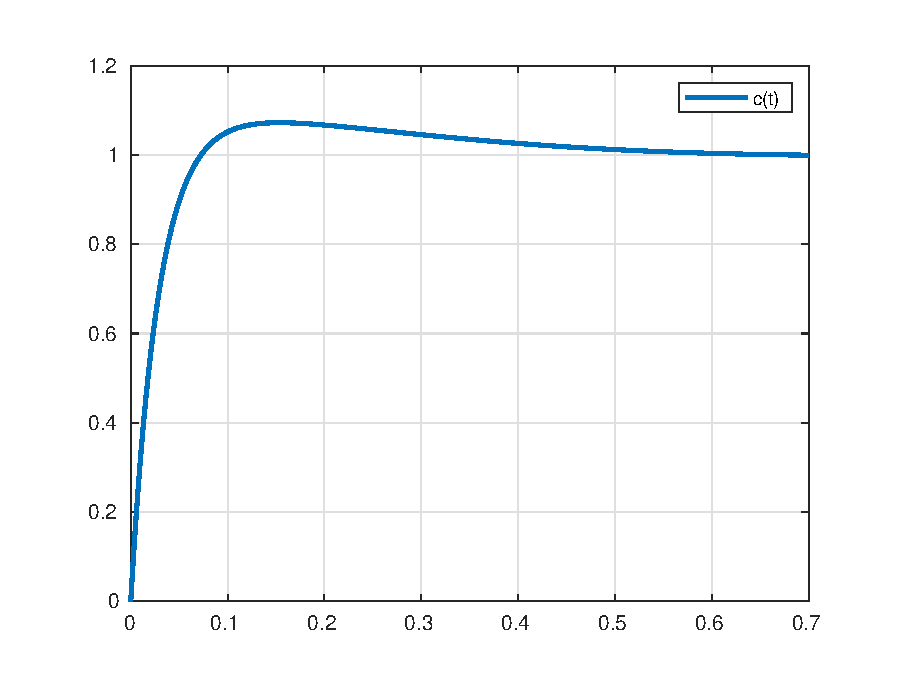
\includegraphics[width = 0.75\linewidth]{Figuras/ProblemaPID/step.eps}
            \caption{Gráfico da resposta ao degrau do sistema}
            \label{fig1a}        
        \end{figure}
    
    \newpage
    \subsection*{b) Determine o LGR  sem e com controlador}
        O lugar geométrico das raízes (LGR) pode ser facilmente obtido através da função \mcode{rlocus} nativa do matlab. 
        O sistema sem o controlador é constituido unicamente da planta do sistema. O LGR do sistema com o controlador, por outro 
        lado, é o produto no domínio ``s'', da FT do controlador com a FT da planta. O bloco de código \ref{LGR}, apresenta o script
        desenvolvido para obtenção dos gráficos.

        \begin{lstlisting}[language=Matlab,label=LGR,caption=LGRs do sistema]
%% Q b)
%LGR sem controlador
figure
rlocus(H)
title('LGR sem controlador')
axis([-6 0.1 -5 5])
grid
%LGR com controlador
figure
rlocus(Gma)
axis([-6 0.1 -5 5])
title('LGR com controlador')
grid     
        \end{lstlisting}
        
        A Figura \ref{fig:LGRsem} apresenta o LGR do sistema sem o controlador e a Figura \ref{fig:LGRcom} apresenta o LGR do sistema com o controlador. 
        
        \begin{figure}[!ht]
            \centering
            \begin{minipage}{0.5\textwidth}
                \centering
                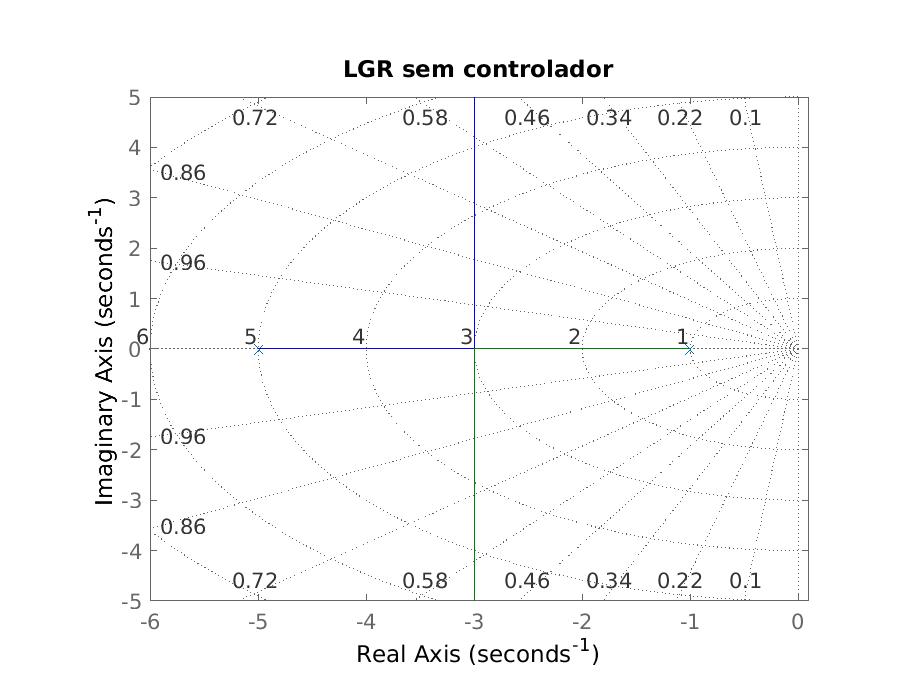
\includegraphics[width=0.9\textwidth]{Figuras/ProblemaPID/LGRsemControladorq1.eps}
                \caption{LGR do sistema sem o controlador}
                \label{fig:LGRsem}
            \end{minipage}\hfill
            \begin{minipage}{0.5\textwidth}
                \centering
                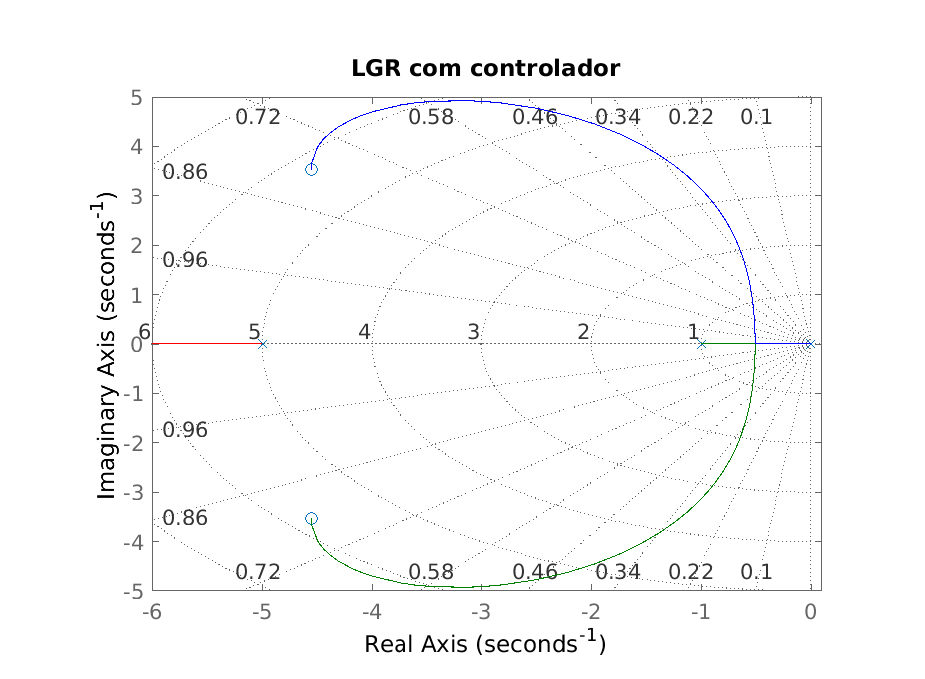
\includegraphics[width=0.9\textwidth]{Figuras/ProblemaPID/LGRcomControladorq1.eps}
                \caption{LGR do sistema com o controlador}
                \label{fig:LGRcom}
            \end{minipage}
        \end{figure}

        %VERIFICAR ADIÇÃO DE COMENTÁRIOS SOBRE O RESULTADO OBTIDO (IMPORTANTE)
    
    \subsection*{c) Determine o tempo de amostragem.}
        O tempo de amostragem pode ser determinado de diferentes formas, desde que seja suficiente para não ocasionar problemas de \textit{aliasing}, ou seja, 
        sobreposição dos espectros. Para isso, sabe-se pelo Teorema de Nyquist que o período de amostragem ``$T_s$'' deve ser tal que a frequência de amostragem ``$f_s$''
        seja o dobro da frequência de corte ``$f_c$'' do sistema, $\frac{1}{T_s} = f_s \ge f_c$.

        O Teorema de Nyquist é bem fundamentado e pode ser amplamente utilizado, porém outra abordagem é amplamente utilizada no ambiente prático, dado a não trivialidade
        da obtenção da frequência de corte do sistema. Sob essa abordagem é feita uma aproximação de que o tempo de amostragem deve ser menor ou igual ao tempo de subida 
        da resposta ao degrau do sistema ``$T_r$'', dividido por dez: $T_s = \frac{T_r}{10}$. Essa será a abordagem utilizada para todas as questões.
        
        O bloco de código \ref{Ts}, apresenta a obtenção do tempo de amostragem. Nesse primeiro momento, verificou-se além do tempo de subida, a frequência de corte do 
        sistema, para corroborar o fato de que o Teorema de Nyquist está sendo cumprido. 

        \begin{lstlisting}[language=Matlab,label=Ts,caption=Tempo de amostragem]
%% Q c)
figure
bode(Gmf)
set(findall(gcf,'type','line'), 'linewidth', 2)
grid
% Tempo de amostragem
Ts = stepinfo(Gmf).RiseTime/10;
        \end{lstlisting}

        O tempo de amostragem é um atributo de nome \mcode{RiseTime} do método nativo \mcode{stepinfo(Gmf)}, dessa forma, pode-se obté-lo utilizando 
        \mcode{stepinfo(Gmf).RiseTime}. 
        O tempo de subida da resposta ao degrau foi de $T_r = 48 \text{ ms}$, então, o tempo de amostragem foi $T_s = 4,8 \text{ ms}$ e a frequência de amostragem
        $f_s = 209.1734 \text{ Hz}$. Ao verificar o diagrama de bode, Figura \ref{DB}, será possível determinar a frequência de corte do sistema. 
    
        \begin{figure}[!h]
            \centering
            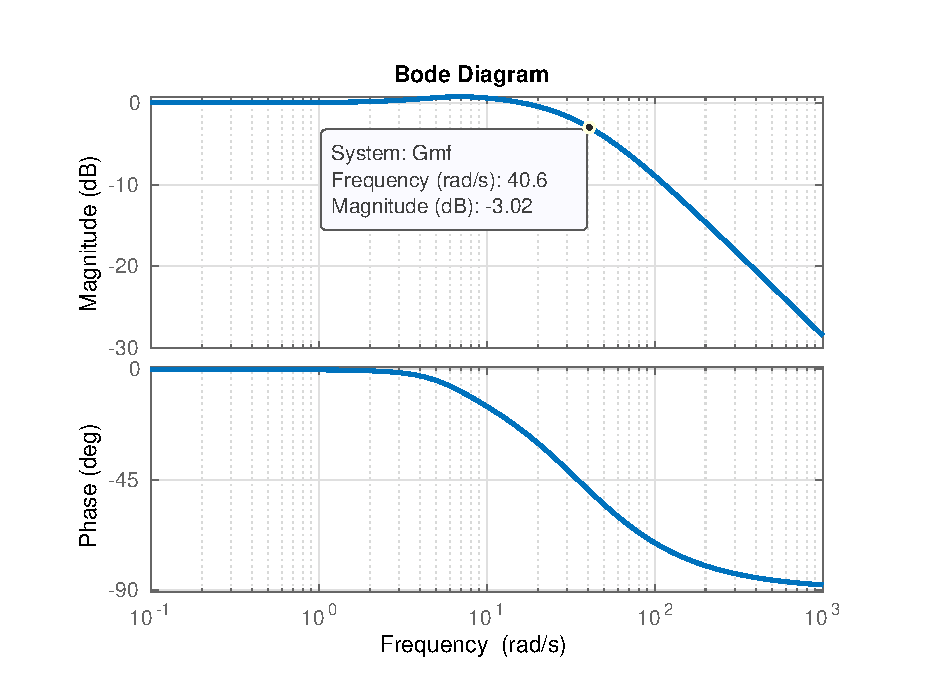
\includegraphics[width = 0.75\linewidth]{Figuras/ProblemaPID/bodeq1c.eps}
            \caption{Diagrama de Bode}
            \label{DB}        
        \end{figure}

        A frequência de corte é aquela no qual o ganho do sistema é de $-3 \text{ dB}$. Pelo gráfico, o ponto está aproximadamente na frequência de corte do sistema 
        $f_c = \frac{\omega_c}{2\pi} = \frac{40.6}{2\pi} = 6.4617 \text{ Hz}$. 
        
        Podemos verificar que a técnica amplamente utilizada em ambientes práticos nos retorna frequências de amostragens muito maiores que a frequência de corte e 
        garantem assim que a discretização esteja satisfazendo ao Teorema de Nyquist. De toda forma, é interessante perceber que ao utilizar a aproximação dada por esse 
        método o nosso resultado não será o mais otimizado e poderá pecar em termos de custo de projeto.
    
        
    \subsection*{d) Discretize o controlador.}
        O controlador PID, é um controlador clássico que no domínio ``s'' de Laplace, é definido 
        pela FT apresentada na equação \ref{eq:PID}

        \begin{equation}
            G_c(s) = kp + \frac{k_i}{s} + k_ds
            \label{eq:PID}
        \end{equation}
        
        Para discretizar o controlador, devemos passar a FT do domínio ``s'' para o domínio discreto 
        `z'', seguindo a correspondência $ s=\frac{1}{T_s}\ln(z)$, em quem ``$T_s$'' é o período de 
        amostragem. Porém, visto que iremos obter resultados não lineares, essa transformação 
        poderá ser custosa computacionalmente. Então, frequentemente são utilizadas aproximações para
        essa equação. Nessa avaliação será utilizado o método de Tustin, também conhecido como 
        aproximação bilinear ou trapezoidal, apresentada pela equação \ref{eq:Tustin}.

        \begin{equation}
            s = \frac{T_s}{2} \cdot \frac{1+z^{-1}}{1-z^{-1}}
            \label{eq:Tustin}
        \end{equation}

        Realizando a substituição da equação \ref{eq:Tustin} em \ref{eq:PID}, obtemos a equação \ref{eq:GcZ}.
        
        \begin{equation}
            G_c(z) = \frac{(k_p+\frac{T_sk_i}{2}+\frac{2k_d}{T_s})z^2 + (T_sk_i-\frac{4K_d}{T_s})z - k_p + \frac{T_sk_i}{2} + \frac{2k_d}{T_s}}
            {z^2-1}
            \label{eq:GcZ}
        \end{equation}

        Ao substituir os valores do tempo de amostragem e dos ganhos $k_p$, $k_i$, $k_d$, na equação \ref{eq:GcZ} obtem-se a
        FT discreta \ref{eq:GcZf}.

        \begin{equation}
            G_c(z) = \frac{(6,451 \cdot 10^4)z^2 - (1,262 \cdot 10^5)z - 6,176 \cdot 10^4}{z^2-1}
            \label{eq:GcZf}
        \end{equation}
        
        A discretização também pode ser realizada através de uma função \mcode{c2d} nativa do Matlab. Utilizando 
        \mcode{c2d(Gc, Ts, 'tustin')} em que \mcode{Gc} foi a função de transferência do controlador no domínio ``s'' e \mcode{Ts}
        o período de amostragem, obteve-se a mesma função de transferência \ref{eq:GcZf}.



    
    \newpage
    \subsection*{e) Realize simulações do sistema em malha fechada e faça uma comparação entre a resposta no tempo contínuo e discreto.}
        A simulação realizada é apresentada através do bloco de código \ref{SMFCD} em que o sistema é discretizado e verifica-se sua resposta
        a uma entrada degrau. Com a finalidade de comparação, foi realizado um gráfico das respostas contínua e discretizada sobrepostas que 
        pode ser visto na Figura \ref{fig:dcs}.   

        \begin{lstlisting}[language=Matlab,label=SMFCD,caption=Simulações do Sistema em MF e em MA.]

Gmfz = c2d(Gmf, Ts, 'zoh');
[yz,tz] = step(Gmfz);
figure
stairs(tz, yz, 'LineWidth', 2);
legend('c(kT)')
grid
%% Q f)
figure
plot(t, y, 'LineWidth', 2)
hold on
stairs(tz, yz, 'LineWidth', 2);
hold off
legend('c(t)', 'c(kT)')
grid
        \end{lstlisting}

        \begin{figure}[!h]
            \centering
            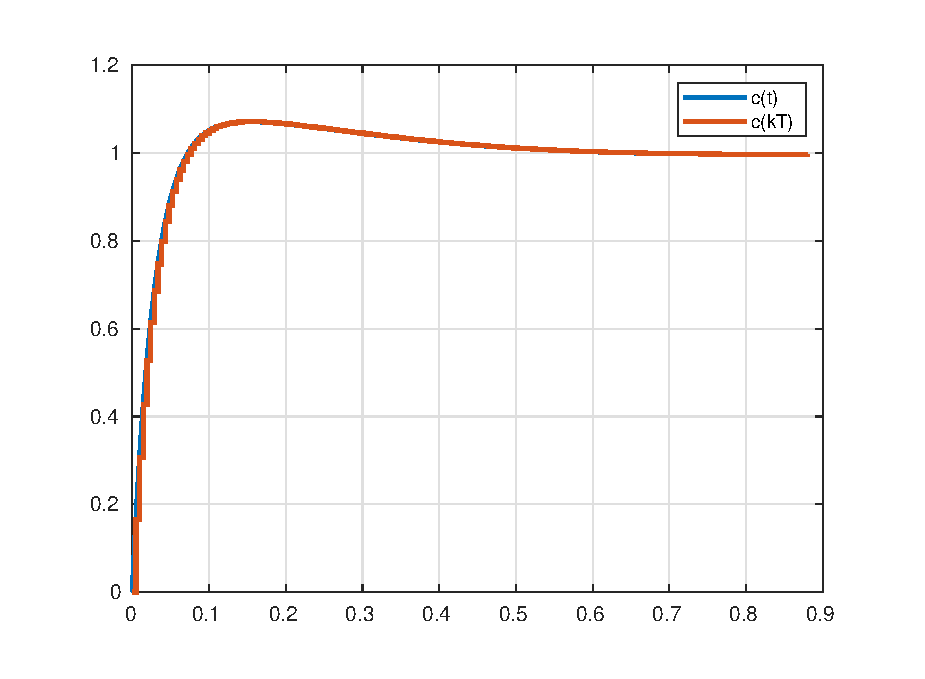
\includegraphics[width = 0.75\linewidth]{Figuras/ProblemaPID/stepcomp.eps}
            \caption{Gráfico das respostas ao degrau dos sistema contínuo e discreto}
            \label{fig:dcs}                   
        \end{figure}

        Além da resposta gráfica, faz-se interessante avaliar numericamente o erro para que seja 
        possível verificar a qualidade da aproximação. Para isso, construiu-se um \textit{script} 
        capaz de calcular o erro absoluto médio percentual (MAPE), que pode ser visto no 
        bloco de código \ref{MAPE}.     
        \newpage
        \begin{lstlisting}[language=Matlab,label=MAPE,caption=Erro Absoluto Médio Percentual]
ape = abs((yz - y(1:length(yz)))/y(1:length(yz))); 
mape = mean(ape(isfinite(ape))); %retira o erro percentual do y=0
        \end{lstlisting}

        Algumas considerações devem ser feitas para compreender o bloco de código \ref{MAPE}. Pela alteração do tempo de amostragem da função step o tamnho 
        dos vetores da saída do sistema em tempo contínuo e em tempo discreto diferem. Portanto, foi necessário realizar um \textit{slice} do maior vetor
        para quee assim fosse possível realizar as operações necessárias.
        
        Junto a isso, como a saída do sistema em $t=0 \text{s}$ é $y(0) = 0$,
        a divisão pelo vetor de saídas gera um elemento que tende ao infinito, para retirá-lo só é realizada a média dos valores finitos através da função 
        \mcode{isfinite} que retorna um vetor de booleanos, em que ``1's'' estarão na posição do vetor que são finitos e ``0's'' na posição dos infinitos.
        Ao fim, obteve-se um MAPE = 0.024\%, um valor muito baixo de erro.


    \subsection*{f) Realize a análise de estabilidade do sistema usando o método de Jury.}  
        O método de Jury permite avaliar a estabilidade de sistemas discretos ao analizar o polinômio característico.
        Existem alguns critérios que devem ser satisfeitos para que o sistema seja estável. Os critérios são: 
        \begin{align*}
            Q(1) &> 0  &\text{(1)}\\
            (-1)^n Q(-1) &> 0 &\text{(2)}\\
            |a_0| &< a_n &\text{(3)}\\
            |b_0| &> b_{n-1} &\text{(4)}\\
            |c_0| &> c_{n-2} &\text{(5)} \\
            &\vdots &\vdots 
        \end{align*} 

        O polinômio característico do sistema
        que está sendo analizado pode ser visto na equação \ref{eq:Q}.

        \begin{equation}
            Q(z) = z^3 - 2.804 z^2 + 2.616 z - 0.8114
            \label{eq:Q}
        \end{equation}
        
        A quantidade de critérios é dada pelo grau do polinômio mais um. Para o nosso caso, em que o polinômio característico é 
        de terceiro grau, são portanto, quatro critérios. 
        
        - O primeiro critério: $Q(1)= 6e-4 > 0$, satisfeito; \\
        - O segundo critério: $-1^3 Q(-1) = 5.2314 > 0$, também trata-se de uma verdade;\\
        - O terceiro critério: $0.8114 < 1$, satisfeito.
        \newpage
        Os  próximos critérios só são possíveis de ser avaliados através da Tabela \ref{tab:J1}. Para nosso caso só é necessário verificar mais um 
        critério. 
        \begin{table}[!ht]
            \centering
            \caption{Análise de estabilidade} 
            \begin{tabular}{l r r r r}
                 & $z^0$ & $z^1$ & $z^2$ & $z^3$\\
                1 & -0{,}8114 & 2{,}616 & -2{,}804 & 1\\
                2 & 1 & -2{,}804 & 2{,}616 & -0{,}8114\\
                3 & -0{,}3408 & 0{,}682 & -0{,}3416 & 0\\
            \end{tabular}                
            \label{tab:J1}
        \end{table}

        - O quarto critério: $0.3416 > 0.3408$, satisfeito. 

         
        
        
\section*{Problemas PI:}

Para os problemas apresentados, realizar:
\begin{enumerate}[label=\alph*)]
    \item Simulação usando MATLAB/Simulink realizando análise dos resultados com relação a estabilidade e 
    resposta dinâmica do sistema
    \item Analisar o LGR sem/com controlador
    \item Determine o tempo de amostragem e realize a discretização dos controladores. Comparar com a
    solução continua.
    \item Discretizar os sistemas (controlador e planta) e analisar a estabilidade usando o método de Jury e
    Routh Hurwitz.
\end{enumerate}
    

\subsection*{Problema 1:}

Para esse problema, o modelo de um motor possui como FT a equação \ref{eq:Gp1}. 

\begin{equation}
    G_p = \frac{4}{s^3+3s^2+10s}
    \label{eq:Gp1}
\end{equation}

A FT de MF, com um controlador proporcional é o visto na equação \ref{eq:Gmf1}.

\begin{equation}
    G_{mf} = \frac{4kp}{s^3+3s^2+10s + 4kp}
    \label{eq:Gmf1}
\end{equation}

Foi visto no desenvolvimento da questão que para o sistema ser estável o ganho propocional deve estar
no intervalo: $0<kp<7,5$. Escolheu-se ter um pólo em -2 e por isso foi determinado $kp = 4$.


\subsubsection*{a)}
    A estabilidade do sistema foi verificada através de uma entrada ao degrau. Pelo desenvolvimento analítico,
    o erro em regime estacionário deve ser zero a uma entrada ao degrau, espera-se obter o mesmo resultado
    pela simulação no MATLAB através do Código \ref{Q1A}.

    \begin{lstlisting}[language=Matlab,label=Q1A,caption=Análise da estabilidade]
%FT sem controlador
num = 4;
den = [1 3 10 0];
G = tf(num,den);
%FT com controlador
kp = 4;
Gmf = tf(kp*num,[1 3 8 4*kp]);

% a)
[y,t] = step(Gmf);
figure
plot(t, y, 'LineWidth', 2);
legend('c(t)')
grid
    \end{lstlisting}

    A Figura \ref{fig:Q1A} apresenta a resposta do sistema ao degrau.


    \begin{figure}[!ht]
        \centering
        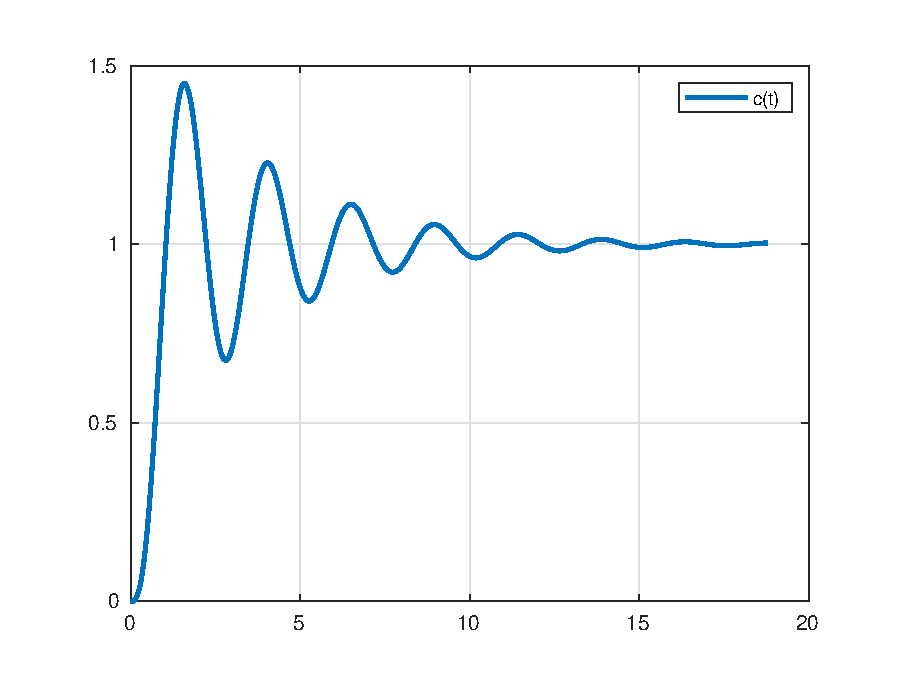
\includegraphics[width = 0.75\linewidth]{Figuras/ProblemasPI/Problema1/step1.eps}
        \caption{Gráfico da resposta ao degrau do sistema}
        \label{fig:Q1A}                   
    \end{figure}

    Podemos verificar que o erro em regime estacionário do sistema tende a zero, assim como determinado 
    através do cálculo analítico. Ainda, podemos verificar que o sistema utilizando um controlador proporcional
    mantém a existência de um sobrevalor percentual.

    Através do \mcode{stepinfo} verifica-se que o sobrevalor percentual é precisamente de 44,93\% e o tempo
    de subida de $T_r =0,6 \text{ s} $. 

\subsubsection*{b)}

    Como já feito anteriormente na avaliação, através da função \mcode{rlocus} é possível traçar o LGR 
    do sistema. A Figura \ref{fig:LGR1Asem} é o LGR do sistema sem o controlador. Pode-se verificar que
    o sistema possui três pólos, com um deles na origem e os outros dois, um par complexo. Como estão 
    no semiplano esquerdo o sistema é estável à resposta ao degrau. Porém o pólo no zero torna o sistema
    mais lento.
    

    \begin{figure}[!ht]
        \centering
        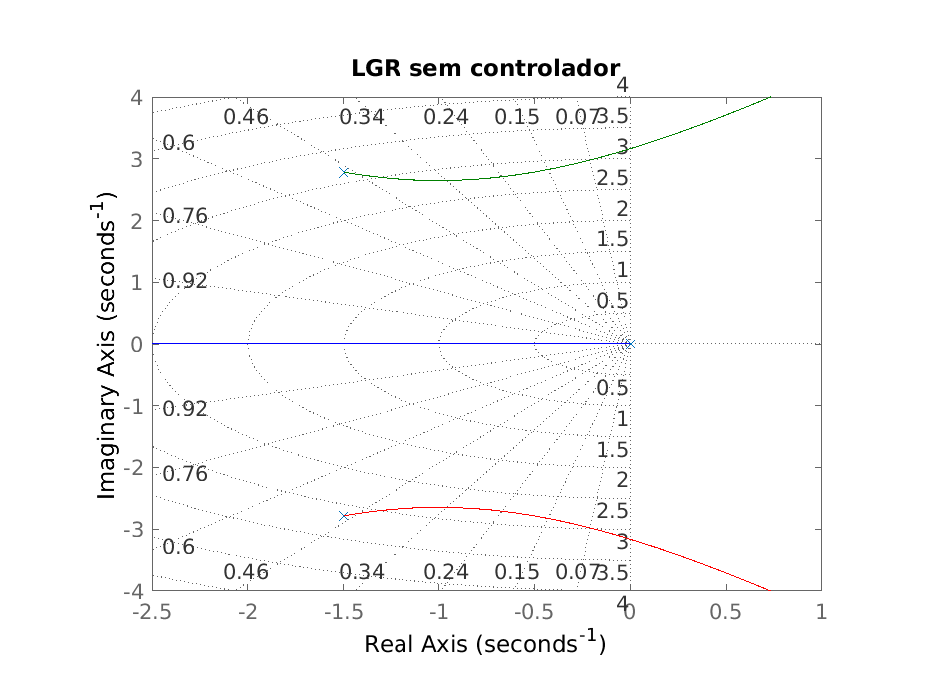
\includegraphics[width = 0.75\linewidth]{Figuras/ProblemasPI/Problema1/LGRsemControlador.eps}
        \caption{Lugar geométrico das raízes sem controlador}
        \label{fig:LGR1Asem}                   
    \end{figure}

    O objetivo do controlador proporcional foi colocar um pólo em -2. Pelo LGR do sistema em MA, o pólo do zero
    é o único que ao variar o ganho se desloca sobre o eixo real. Pode-se verificar através da Figura  
    \ref{fig:LGR1Acom} que o objetivo foi alcançado.

    \begin{figure}[!ht]
        \centering
        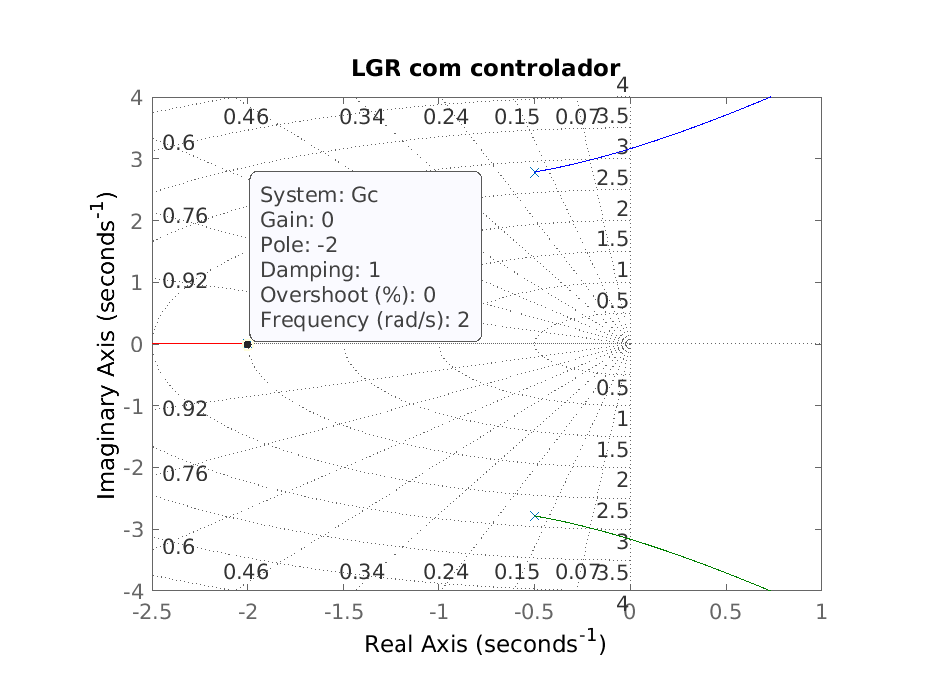
\includegraphics[width = 0.75\linewidth]{Figuras/ProblemasPI/Problema1/LGRcomControlador.eps}
        \caption{Lugar geométrico das raízes com controlador}
        \label{fig:LGR1Acom}                   
    \end{figure}

\newpage    
\subsubsection*{c)}

    Como anteriormente, o tempo de amostragem foi determinado pelo tempo de subida divido por dez. 
    O sistema foi discretizado utilizando o segurador de ordem zero (ZoH). O Código \ref{Q1C} apresenta
    a discretização do modelo e a criação do gráfico da resposta do sistema a entrada degrau.

    \begin{lstlisting}[language=Matlab,label=Q1C,caption=Análise da estabilidade]
Ts = stepinfo(Gmf).RiseTime/10; %Tr = 0.6000
Gmfz = c2d(Gmf,Ts, 'zoh');
[yz,tz] = step(Gmfz); %salvando resultado do step

figure %fazendo uma figura para comparar
plot(t, y, 'LineWidth', 2)
hold on
stairs(tz, yz, 'LineWidth', 2);
hold off
legend('c(t)', 'c(kT)')
grid

%utilizando MAPE para avaliacao numerica
ape = abs((yz - y(1:length(yz)))/y(1:length(yz))); 
mape = mean(ape(isfinite(ape))); %retira o erro percentual do y=0
%mape = 3.2708e-04
    \end{lstlisting}

O tempo de amostragem obtido foi de 60 ms. A FT em MF disceta é apresentada na equação \ref{eq:Gmfz1}
A Figura \ref{fig:Stepctds} apresenta a resposta dos sistema
contínuo e discretizado sobrepostos. 

\begin{equation}
    G_{mf}(z) = \frac{0.0005503 z^2 + 0.002103 z + 0.0005029}{z^3 - 2.807 z^2 + 2.646 z - 0.8353}
    \label{eq:Gmfz1}
\end{equation}


\begin{figure}[!h]
    \centering
    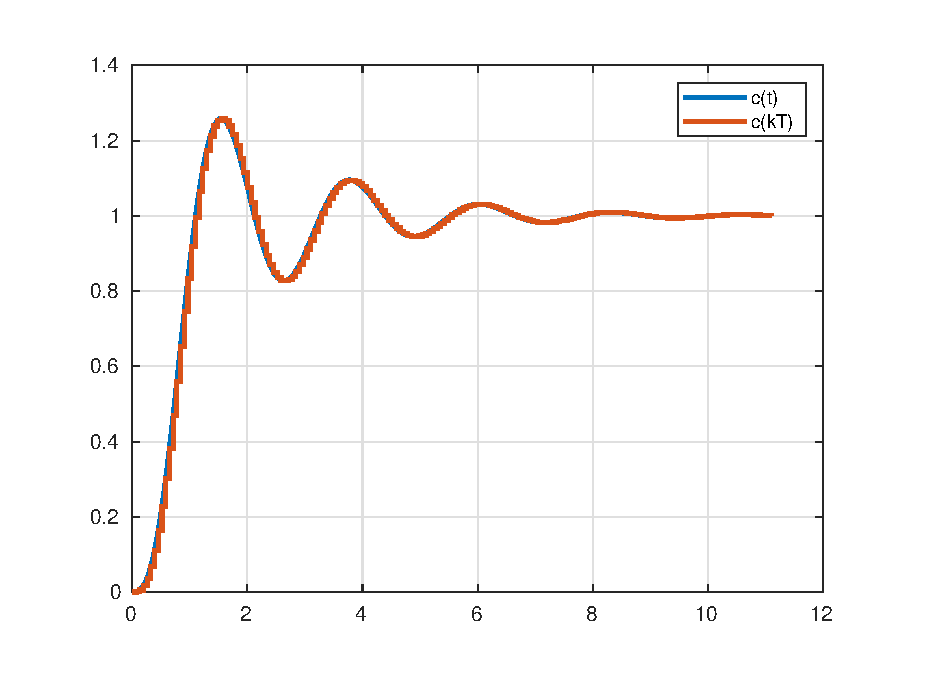
\includegraphics[width = 0.75\linewidth]{Figuras/ProblemasPI/Problema1/resposta_ao_degrau.eps}
    \caption{Lugar geométrico das raízes com controlador}
    \label{fig:Stepctds}                   
\end{figure}

Visualmente o sistema discreto se aproxima da resposta contínua. Porém, como vem sendo feito nessa 
avaliação, verificamos a qualidade da discretização através do MAPE. Para essa discretização o 
MAPE foi de $3,27 \cdot 10^{-2}$ \%. Um baixo valor de erro.

\subsubsection*{d)}

O polinômio característico do sistema contínuo pode ser visto na equação \ref{eq:pcsc1}. O método
de Routh consiste em verificar se há mudança de sinal na primeira coluna da tabela, se não ocorre
o sistema será estável, se ocorrer, instável. A Tabela \ref{tab:RE1} apresenta o desenvolvimento do
resultado obtido 

\begin{equation}
    Q(s) = s^3+3s^2+10s+16
    \label{eq:pcsc1}
\end{equation}

\begin{table}[!ht]
    \centering
    \vspace{0.5cm}
    \caption{Análise de estabilidade pelo método de Routh} 
    \begin{tabular}{r|lr}
        
        1 & 1 & 10 \\
        2 & 3 & 16 \\
        3 & 4{,}67\\
    \end{tabular}                
    \label{tab:RE1}
\end{table}

Verificamos que o sistema contínuo é estável.

O polinômio característico do sistema discreto pode ser visto na equação \ref{eq:pcsd1}.

\begin{equation}
    Q(z) = z^3 - 2.807 z^2 + 2.646 z - 0.8353
    \label{eq:pcsd1}
\end{equation}

A Tabela \ref{tab:JE1} apresenta o desenvolvimento do método de Jury para esse sistema.

\begin{table}[!ht]
    \centering
    \caption{Análise de estabilidade} 
    \begin{tabular}{l| r r r r}
         & $z^0$ & $z^1$ & $z^2$ & $z^3$\\
        \hline
        1 & -0{,}8353 & 2{,}646 & -2{,}807 & 1\\
        2 & 1 & -2{,}807 & 2{,}646 & -0{,}8353\\
        3 & -0{,}3013 & 0{,}5968 & -0{,}3023 & 0\\
    \end{tabular}                
    \label{tab:JE1}
\end{table}

Para verificar a estabilidade, como nosso polinômio é de ordem 3, devemos conferir os 4 critérios.

- O primeiro critério: $Q(1)= 3,7 \cdot 10^{-3} > 0$, satisfeito; \\
- O segundo critério: $-1^3 Q(-1) = 7,2883 > 0$, satisfeito;\\
- O terceiro critério: $|a_0| = 0,8353 < 1 = |a_3|$, satisfeito; \\
- O quarto critério: $|b_0| = 0,3023 > 0,3408 = |b_3| $, satisfeito. 

Como o sistema discreto atende os quatro critérios de Jury necessários, é um sistema estável.

\subsection*{Problema 2:}

\end{document}
